% -*- coding: utf-8 -*-

\newcommand{\commentaire}[1]{}

\entete{Travaux dirigés 2 : affectation.}

\section{Un premier programme C}


\begin{figure}[h]
  \centering
  \shortstack{Programme C\\
    \fbox{\quad
      \begin{minipage}[b]{.68\linewidth}
        \small \listinginput{1}{affectations.c}
      \end{minipage}}}\hfill
  \shortstack{Traduction\\
    \fbox{\quad
      \begin{minipage}[b]{.22\linewidth}
        \small \listinginput{1}{affectations.ail}
      \end{minipage}}}
\caption{Un programme C et sa traduction machine}
\label{fig:programmes}
\end{figure}

\begin{figure}[h]
  \centering
  \subtable[Trace en C]{
    \begin{tabular}[h]{|r|c|c| l |}
      \hline
      Ligne & x & y & sortie \\ \hline
      initialisation & 5 & ? & \\ \hline
      15 & & 2 & \\ \hline
      16 & 2 &  & \\ \hline
19 & \multicolumn{3}{|c|}{renvoie \C{EXIT\_SUCCESS}}\\ \hline
   \end{tabular}
    \label{tab:traceC}
  }
  \subtable[Trace amil]{
    \begin{tabular}[c]{l||c|c|c|c|c|}
\hline
 \emph{Instructions} & Cycles & CP& r0& 10& 11\\ \hline
\hfill Initialisation & 0 & 1 & ? & 5
 & ?
 \\ \hline \commentaire{Initialisation du registre 0 à 2
} \C{valeur 2 r0
} & 1 & 2  & 2 & &\\ \hline
 \commentaire{Écriture du registre 0 à l'adresse 11
} \C{ecriture r0 11
} & 2 & 3  & & & 2
\\ \hline
 \commentaire{Lecture de la donnée d'adresse 11 dans le registre 0
} \C{lecture 11 r0
} & 3 & 4  & 2 & &\\ \hline
 \commentaire{Écriture du registre 0 à l'adresse 10
} \C{ecriture r0 10
} & 4 & 5  & & 2
 &\\ \hline
 \commentaire{Fin du processus.
} \C{stop
} & 5 & 6  & & &\\ \hline
\end{tabular}
    \label{tab:traceamil}
  }  
  \caption{Traces}
\label{fig:traces}
\end{figure}

Voici, figure~\ref{fig:programmes}, un premier programme C. Le langage C sera présenté au prochain cours. Pour le moment voici ce que vous avez à savoir. 

Un programme en langage C est donné sous forme de texte, \emph{le source}, et il doit passer par une étape de traduction avant de pouvoir être exécuté par le processeur. Nous donnons ici une traduction sous forme d'instructions amil. Il s'agit d'un artifice pédagogique, la traduction réelle en code binaire exécutable est plus compliquée.  Par analogie avec la musique, le source est la partition, et le fichier exécutable est le morceau musical (codé sur le support adapté au système de lecture : un fichier mp3, un CD, etc.). La traduction est effectuée par un ensemble de programmes (et non par des musiciens), le source doit donc obéir à des règles syntaxiques précises.  

Les textes entre \C{/*} et \C{*/} sont des \emph{commentaires}, ils ne feront pas partie du programme exécutable, ils servent aux humains qui manipulent les programmes. Les commentaires du programme figure~\ref{fig:programmes} vous serviront au cours du semestre à structurer tous vos programmes C.

Tout programme C comporte une fonction principale, le \C{main()}, qui sert de point d'entrée au programme. Cette fonction doit se terminer par l'instruction \verb+return EXIT_SUCCESS+. En renvoyant cette valeur, le \C{main} signale au système d'exploitation la terminaison correcte du programme.

Une \emph{variable} est un symbole (habituellement un nom) qui renvoie à une position de mémoire dont le contenu peut prendre successivement différentes valeurs pendant l'exécution d'un programme\footnote{\url{http://fr.wikipedia.org/wiki/Variable}}.

L'instruction \C{int x = 5} déclare une variable \C{x} et fixe sa valeur initiale à 5. Le mot clé \C{int} signifie que cette variable contiendra un entier. Dans le code amil correspondant \C{x} renvoie à l'adresse \C{10} où se trouve intialement la valeur \C{5}.

L'instruction \C{int y} déclare une variable entière \C{y} sans l'initialiser. L'effet de cette déclaration est de réserver un espace mémoire pour y stocker un entier. 

Le signe égal (\C{=}) a un sens bien particulier, il dénote une \emph{affectation}. L'objectif de ce TD est de bien comprendre l'affectation.  La partie à gauche du signe égal doit désigner un espace mémoire, c'est typiquement une variable. La partie à droite du signe égal est une expression dont la valeur sera évaluée et écrite à l'adresse à laquelle renvoie la partie gauche. Par exemple, \C{y = 2} a été traduit en code machine par une instruction évaluant l'expression \C{2} dans un registre (ici \C{valeur 2 r0}), et par une instruction d'écriture de la valeur trouvée dans la mémoire réservée à \C{y}. Une variable s'évalue comme sa valeur (celle contenue dans la mémoire correspondante, au moment de l'évaluation).

\subsection{Questions}
\begin{enumerate}
\item Quel espace mémoire a été reservé pour \C{y} dans le code amil ?
  \begin{correction}
L'adresse 11.    
  \end{correction}
\item Comment a été traduite l'instruction d'affectation \C{x = y} en amil ?
  \begin{correction}
Lignes 3 et 4 :
\begin{verbatim}
lecture 11 r0
ecriture r0 10    
\end{verbatim}
  \end{correction}
\item Si il y avait \C{y = x + 2}, ligne 15 dans le programme C, à la place de \C{y = 2}, quel serait le code amil correspondant ?
  \begin{correction}
Ne pas se préocupper du décalage des lignes de code amil.
\begin{verbatim}
    lecture 10 r0
    valeur 2 r1
    add r1 r0
    ecriture r0 11
\end{verbatim}
  \end{correction}
\end{enumerate}



\section{Échange de valeurs}

\subsection{Introduction au problème}

Nous avons deux tableaux anciens, chacun accroché à un clou, et un
troisième clou, libre, sur le mur d'une exposition.
Pour des critères esthétiques, nous voulons changer de place nos deux tableaux sans les mettre par terre, car cela risquerait d'abîmer nos précieuses toiles... Comment faire ? 
\begin{figure}[h!]
    \begin{center}
        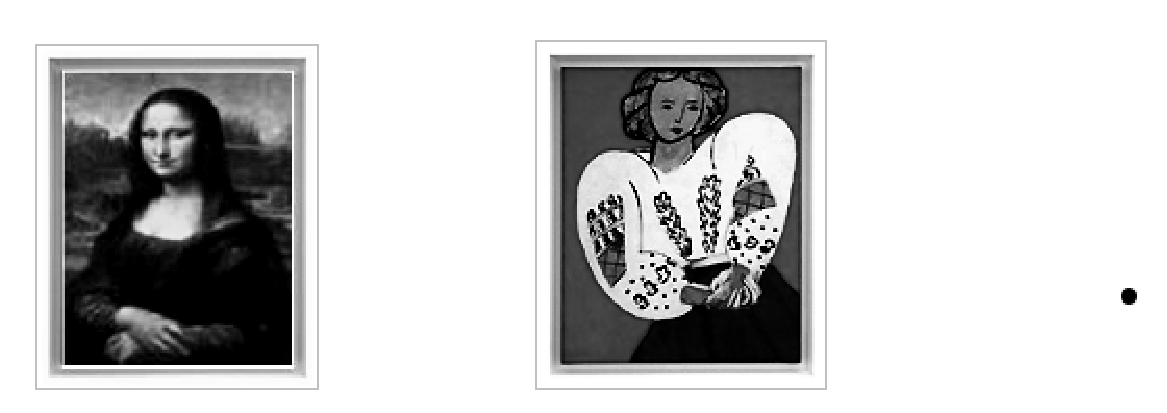
\includegraphics[scale=.8]{tableaux.eps}
    \end{center}
    \caption{Échanger les deux tableaux en utilisant le clou libre...}
    \label{fig:ex_onto}
\end{figure}

\begin{correction}
\begin{verbatim}
/* tableau 1 (clou 1) -> clou 3 */
/* tableau 2 (clou 2) -> clou 1 */
/* tableau 1 (clou 3) -> clou 2 */
\end{verbatim}
\end{correction}

\subsection{Échange des valeurs de deux variables en C}

\begin{enumerate}
\item 
  Écrire un programme C qui déclare et initialise deux variables
  entières \C{x} et \C{y} et effectue la permutation de ces deux
  valeurs. Commencer par écrire un algorithme, à l'aide de phrases telles que << Copier la valeur de la variable ... dans la variable ...>>, en vous inspirant de la question précédente.
\begin{correction}
L'agorithme doit être utilisé pour structurer le code. On ne donne pas ici de valeur à $x$ et $y$, mais n'hésitez pas à en donner (par initialisation par exemple). 

{\small
\listinginput{1}{echange.c}
}
\end{correction}

\item Traduire ce programme C en un programme amil. On supposera que les deux variables sont stockées aux adresses \C{10} et \C{11}.
  \begin{correction}
    À nouveau, l'algorithme est à utiliser en commentaires pour
      structurer le code.
\begin{verbatim}
# copie de la case d'adresse 10 dans une case auxillaire (12)
 1 lecture 10 r0
 2 ecriture r0 12
# copie de la case d'adresse 11 à l'adresse 10
 3 lecture 11 r0
 4 ecriture r0 10
# copie de la case auxillaire à l'adresse 11
 5 lecture 12 r0
 6 ecriture r0 11
 7 stop
 9 
10 4
11 5
12 ?
\end{verbatim}
  \end{correction}
\item Exécuter ces programmes sur un exemple (faire les traces).
\begin{correction}
 \begin{figure}
  \centering
  \begin{tabular}[c]{|c|c|c|c|c|c|c|}
\hline
Cycles & CP & instruction & r0& 10& 11& 12\\ \hline
INIT & 1 & & ? & 4
 & 5
 & ?
 \\ \hline1 & 2 & \commentaire{Lecture de la donnée d'adresse 10 dans le registre 0
} lecture 10 r0
 & 4 & & & \\ \hline
2 & 3 & \commentaire{Écriture du registre 0 à l'adresse 12
} ecriture r0 12
 & & & & 4
 \\ \hline
3 & 4 & \commentaire{Lecture de la donnée d'adresse 11 dans le registre 0
} lecture 11 r0
 & 5 & & & \\ \hline
4 & 5 & \commentaire{Écriture du registre 0 à l'adresse 10
} ecriture r0 10
 & & 5
 & & \\ \hline
5 & 6 & \commentaire{Lecture de la donnée d'adresse 12 dans le registre 0
} lecture 12 r0
 & 4 & & & \\ \hline
6 & 7 & \commentaire{Écriture du registre 0 à l'adresse 11
} ecriture r0 11
 & & & 4
 & \\ \hline
7 & 8 & \commentaire{Fin du processus.
} stop
 & & & & \\ \hline
\end{tabular}
  \caption{Simulation de l'échange de deux valeurs en mémoire (4 et 5)}
  \label{simmax1}
\end{figure}
  \end{correction}
\item (Facultatif). Donner d'autres solutions en assembleur à ce problème (la permutation des contenus des adresses \C{10} et \C{11}).
  \begin{correction}
Par exemple : 
\begin{verbatim}
# copie de la case d'adresse 10 dans un registre pour sauvegarde
1    lecture 10 r1
# copie de la case d'adresse 11 à l'adresse 10
2    lecture 11 r0
3    ecriture r0 10
# copie de a dans registre de sauvegarde à l'adresse 11
4    ecriture r1 11
5    stop
\end{verbatim}
\begin{figure}
  \centering
  \begin{tabular}[c]{|c|c|c|c|c|c|c|}
\hline
Cycles & CP & instruction & r0& r1& 10& 11\\ \hline
INIT & 1 & & ? & ? & 4
 & 5
 \\ \hline1 & 2 & \commentaire{Lecture de la donnée d'adresse 10 dans le registre 1
} lecture 10 r1
 & & 4 & & \\ \hline
2 & 3 & \commentaire{Lecture de la donnée d'adresse 11 dans le registre 0
} lecture 11 r0
 & 5 & & & \\ \hline
3 & 4 & \commentaire{Écriture du registre 0 à l'adresse 10
} ecriture r0 10
 & & & 5
 & \\ \hline
4 & 5 & \commentaire{Écriture du registre 1 à l'adresse 11
} ecriture r1 11
 & & & & 4
 \\ \hline
5 & 6 & \commentaire{Fin du processus.
} stop
 & & & & \\ \hline
\end{tabular}
  \caption{Simulation de l'échange de deux valeurs en mémoire (4 et 5), avec un second registre}
  \label{simmax1}
\end{figure}
  \end{correction}

\item (Facultatif). Mêmes questions que précédemment mais pour faire une permutation
  circulaire de 3 valeurs.

  \begin{correction}    


{\small
\listinginput{1}{echange3.c}
}

Sans le second registre (traduction) :
\begin{verbatim}
lecture 10 r0  
ecriture r0 13 
lecture 11 r0  
ecriture r0 10 
lecture 12 r0  
ecriture r0 11 
lecture 13 r0  
ecriture r0 12 
stop
\end{verbatim}
Avec le second registre :
\begin{verbatim}
lecture 10 r1  
lecture 11 r0  
ecriture r0 10 
lecture 12 r0  
ecriture r0 11 
ecriture r1 12 
stop
\end{verbatim}
\end{correction}
\end{enumerate}

%\subsection{Pour essayer en TP}


%%% Local Variables: 
%%% mode: latex
%%% TeX-master: "td2"
%%% End: 
